\documentclass[a4paper,14pt]{article}

\usepackage{comment} % Para comentar várias linhas ao mesmo tempo

%matemática
\usepackage{amsmath}
\usepackage{amssymb}

%diagramação
\usepackage{extsizes}
\everymath{\displaystyle}
\usepackage{geometry}
\usepackage{fancyhdr}
\usepackage{multicol}
\usepackage{graphicx}
\usepackage[brazil]{babel}
\usepackage[shortlabels]{enumitem}
\usepackage{cancel}
\usepackage{textcomp}
\usepackage{tcolorbox}

%tabelas
\usepackage{array} % Para melhor formatação de tabelas
\usepackage{longtable}
\usepackage{booktabs}  % Para linhas horizontais mais bonitas
\usepackage{float}   % Para usar o modificador [H]
\usepackage{caption} % Para usar legendas em tabelas
\usepackage{wrapfig} % Para usar tabelas e figuras flutuantes

\begin{comment}
%tikzpicture
\usepackage{tikz}
\usepackage{scalerel}
\usepackage{pict2e}
\usepackage{tkz-euclide}
\usetikzlibrary{calc}
\usetikzlibrary{patterns,arrows.meta}
\usetikzlibrary{shadows}
\usetikzlibrary{external}
\end{comment}
	
%pgfplots
\usepackage{pgfplots}
\pgfplotsset{compat=newest}
\usepgfplotslibrary{statistics}
\usepgfplotslibrary{fillbetween}

%colours
\usepackage{xcolor}



\columnsep=2cm
\hoffset=0cm
\textwidth=8cm
\setlength{\columnseprule}{.1pt}
\setlength{\columnsep}{2cm}
\renewcommand{\headrulewidth}{0pt}
\geometry{top=1in, bottom=1in, left=0.7in, right=0.5in}

\pagestyle{fancy}
\fancyhf{}
\fancyfoot[C]{\thepage}

\begin{document}
	
	\noindent\textbf{6FMA73 - Matemática} 
	
	\begin{center}Diferença, complemento e complementar de $A$ em relação a $B$ (Versão estudante)
	\end{center}
	
	\noindent\textbf{Nome:} \underline{\hspace{10cm}}
	\noindent\textbf{Data:} \underline{\hspace{4cm}}
	
	%\section*{Questões de Matemática}
	
	\begin{multicols}{2}
		\noindent Sendo $A$ e $B$ subconjuntos de um universo $U$, a diferença de $A$ por $B (A - B)$ é formada pelos elementos de $A$ que não pertencem a $B$. \\
		Se $A$ é um subconjunto de um universo $U$, o complemento de $A(\overline{A})$ é formado pelos elementos do universo que não são elementos de $A$. \\
		Sejam $A$ e $B$ subconjuntos de um universo $U$, tal que $A$ é subconjunto de $B$. O complementar de $A$ em relação a $B$ ($C_B^{A}$) é formado pelos elementos de $B$ que não pertencem a $A$.
		\noindent\textsubscript{--------------------------------------------------------------------------}
    	\begin{enumerate}
   			\item Dados $A$ e $B$, apresente $A - B$ e $B - A$.
   			\begin{enumerate}[a)]
   				\item $A = \{5, 6, 7\}; B = \{4, 6, 8\}$ \\\\\\\\\\\\\\\\
   				\item $A = \{a, b\}; B = \{a, b, c, d\}$ \\\\\\\\\\\\\\\\
   				\item $A = \varnothing, B = \{1, 2, 3, 4\}$ \\\\\\\\\\\\\\\\
   			\end{enumerate}
   			\item Destaque $B - A$
   			\begin{enumerate}[a)]
   				\item ~ \\ 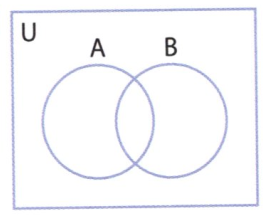
\includegraphics[width=1\linewidth]{6FMA73_imagens/imagem01}
   				\item ~ \\
   				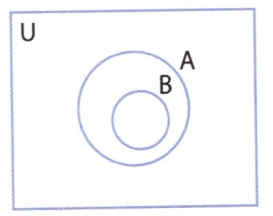
\includegraphics[width=1\linewidth]{6FMA73_imagens/imagem02} \newpage
   				\item ~ \\
   				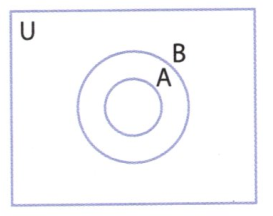
\includegraphics[width=1\linewidth]{6FMA73_imagens/imagem03}
   				\item ~ \\
   				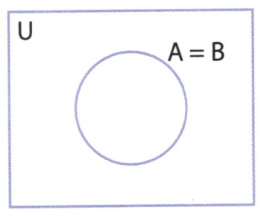
\includegraphics[width=1\linewidth]{6FMA73_imagens/imagem04}
   				\item ~ \\
   				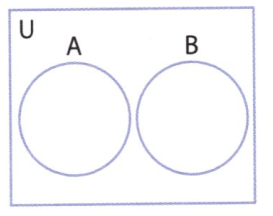
\includegraphics[width=1\linewidth]{6FMA73_imagens/imagem05}
   			\end{enumerate}
   			\item No universo $U = \{1, 3, 5, 7, 9, 11\}$, apresente o complemento de cada um dos conjuntos.
   			\begin{enumerate}[a)]
   				\item $A = \{3\}$ \\\\\\\\
   				\item $B = \{5, 9, 11\}$ \\\\\\\\
   				\item $C = \{1, 3, 5, 7, 9. 11\}$ \\\\\\\\
   				\item $D = \varnothing$ \\\\\\\\
   			\end{enumerate}
   			\item Destaque $\overline{B}$.
   			\begin{enumerate}[a)]
   				\item ~ \\ 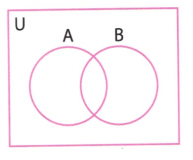
\includegraphics[width=1\linewidth]{6FMA73_imagens/imagem06}
   				\item ~ \\
   				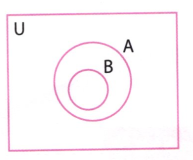
\includegraphics[width=1\linewidth]{6FMA73_imagens/imagem07} \newpage
   				\item ~ \\
   				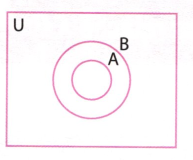
\includegraphics[width=1\linewidth]{6FMA73_imagens/imagem08}
   				\item ~ \\
   				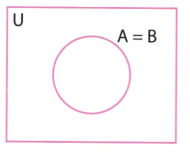
\includegraphics[width=1\linewidth]{6FMA73_imagens/imagem09}
   				\item ~ \\
   				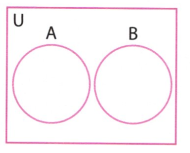
\includegraphics[width=1\linewidth]{6FMA73_imagens/imagem10}
   			\end{enumerate}
   			\item Dados $A$ e $B$, apresente $C^{A}_B$:
   			\begin{enumerate}[a)]
   				\item $A = \{2, 4, 6\}; \\ B = \{1, 2, 3, 4, 5, 6\}$ \\\\\\\\\\\\
   				\item $A = \{3, 5, 7\}; \\ B = \{3, 4, 5, 6, 7\}$ \\\\\\\\\\
   				\item $A = \mathbb{N}; B = \mathbb{Z}$ \\\\\\\\\\
   			\end{enumerate}
   			%5 a 8
   			\item Sejam $A = \{6, 7, 8\}, B = \{8, 10, 12\}, C = \{5, 6, 9, 11, 12\}$ e $U = \{5, 6, 7, 8, 9, 10, 11, 12\}$. Encontre:
   			\begin{enumerate}[a)]
   				\item $A - B$ \\\\\\
   				\item $B - A$ \\\\\\
   				\item $\overline{A}$ \\\\\\
   				\item $\overline{B \cap C}$ \\\\\\
   				\item $\overline{A \cup B \cup C}$ \\\\\\
   				\item $\overline{B - C}$ \newline
   				\item $A - (B - C)$ \\\\\\
   				\item $(A - B) - C$ \\\\\\
   				\item $(A - B) \cup (B - C)$ \\\\\\
   				\item $(A - B) \cup (B - A)$ \\\\\\
   				\item $(B - C) \cup (C - B)$ \\\\\\
   				\item $A - (B \cap C)$ \\\\\\
   				\item $(B - C) - A$ \\\\\\
   				\item $(A \cup B) - C$ \\\\\\
   				\item $A \cup (B - C)$ \\\\\\
   			\end{enumerate}
   			\item Destaque:
   			\begin{enumerate}[a)]
   				\item $\overline{A} \cap \overline{B}$ \\
   				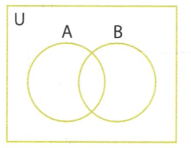
\includegraphics[width=1\linewidth]{6FMA73_imagens/imagem11}
   				\item $\overline{A \cap B}$ \\
   				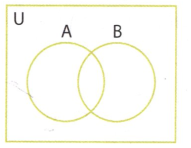
\includegraphics[width=1\linewidth]{6FMA73_imagens/imagem12}
   				\item $(A - B) \cup (B - A)$ \\
   				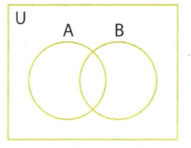
\includegraphics[width=1\linewidth]{6FMA73_imagens/imagem13}
   				\item $(A \cap C) - B$ \\
   				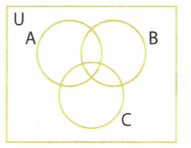
\includegraphics[width=1\linewidth]{6FMA73_imagens/imagem14}
   				\item $A - \overline{B \cap C}$ \\
   				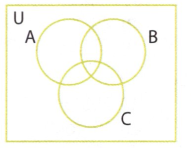
\includegraphics[width=1\linewidth]{6FMA73_imagens/imagem15}
   				\item $(B \cap C) - (A \cap B)$ \\
   				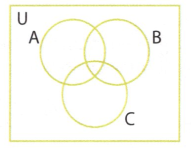
\includegraphics[width=1\linewidth]{6FMA73_imagens/imagem16}
   				\item $(A - B) \cap C$ \\
   				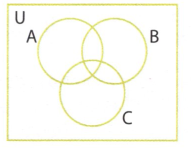
\includegraphics[width=1\linewidth]{6FMA73_imagens/imagem17}
   				\item $A \cap \overline{B \cap C}$ \\
   				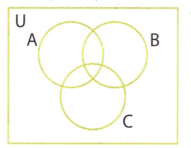
\includegraphics[width=1\linewidth]{6FMA73_imagens/imagem18}
   				\item $((A - C) - B) \cup (B \cap C)$ \\
   				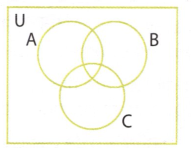
\includegraphics[width=1\linewidth]{6FMA73_imagens/imagem19}
   			\end{enumerate}
   			\item Sendo $A - B = \{1, 4, 7\}$, $B - A = \{3, 6\}$ e $A \cap B = \{2, 5\}$ determine $A, B$ e $A \cup B$.  \\\\\\\\\\\\\\\\
   			\item Utilize diagramas de Venn para mostrar que:
   			\begin{enumerate}[a)]
   				\item $(A - B) \cup (B - A) = (A \cup B) - (A \cap B)$ \newpage
   				\item $\overline{A \cup B} = \overline{A} \cap \overline{B}$ \\\\\\\\\\\\\\\\\\\\
   				\item $\overline{A \cap B} = \overline{A} \cup \overline{B}$
   			\end{enumerate}
   		\end{enumerate}
        $~$ \\ $~$ \\ $~$ \\ $~$ \\ $~$ \\ $~$ \\ $~$ \\ $~$ \\ $~$ \\ $~$ \\ $~$ \\ $~$ \\ $~$ \\ $~$ \\ $~$ \\ $~$ \\ $~$ \\ $~$ \\ $~$ \\ $~$ \\ $~$ \\ $~$ \\ $~$ \\ $~$ \\ $~$ \\ $~$ \\ $~$ \\ $~$ \\ $~$ \\ $~$ \\ $~$ \\ $~$ \\ $~$ \\ $~$ \\ $~$ \\ $~$ \\ $~$ \\ $~$ \\ $~$ \\ $~$ \\ $~$ \\ $~$ \\ $~$ \\ $~$ \\ $~$ \\ $~$ \\ $~$ \\ $~$ \\ $~$ \\ $~$ \\ $~$ \\ $~$ \\ $~$ \\ $~$ \\ $~$ \\ $~$ \\ $~$ \\ $~$ \\ $~$ \\ $~$ \\ $~$ \\ $~$ \\ $~$ \\ $~$ \\ $~$ \\ $~$ \\ $~$ \\ $~$ \\ $~$ \\ $~$ \\ $~$	
	\end{multicols}
\end{document}